\chapter{Analisi del problema e descrizione della soluzione proposta}

\section{Analisi del problema}

\index{Analisi del problema}

Questo primo assignment prevede la progettazione e la creazione di un piano cartesiano su cui N particelle interagiscono tra di loro con forza repulsiva.
Per tanto vi � l'esigenza di calcolare la forza repulsiva che ogni particella ha rispetto alle altre ed aggiornare la sua posizione.\\
Il tutto deve essere rappresentato e visualizzato su una GUI che permette di lanciare e fermare la suddetta simulazione.
Il punto principale di questa esercitazione consiste nel riuscire a progettare la simulazione basandosi su un modello di concorrenza multi-threaded.\\

Le problematiche che sopraggiungono con questo modello sono: prima di tutto capire e analizzare quali possono essere i compiti che i threads devono svolgere; in secondo luogo gestire la sincronizzazione e l'eventuale mutua esclusione dei vari threads che si andranno ad utilizzare.

\section{Soluzione proposta}

\index{Soluzione proposta}

\subsection{Pattern MVC}

Il programma � stato sviluppato seguendo il pattern MVC:
\begin{itemize}
\item Model: si occupa della gestione della logica delle particelle;
\item View: rappresenta graficamente le particelle ed il loro movimento sul piano cartesiano;
\item Controller: incapsula il comportamento dell'applicazione gestendo la sincronizzazione della logica delle particelle e la loro rappresentazione sul piano.
\end{itemize}

\subsection{Modello multi-threaded}

Il programma � stato decomposto in N thread-worker ed un thread-master. Quest'ultimo, ad ogni step, aggiorna l'elenco delle particelle con le nuove posizioni appena calcolate dai thread-worker e notifica alla view tale cambiamento.\\
I thread-worker hanno il compito di calcolare i dati che permettono di aggiornare la posizione delle particella.\\

\medskip
A questo scopo sono stati utilizzati due semafori: 
\begin{enumerate}
\item \textbf{masterTurn}: pu� assumere solamente due valori. Il thread master deve acquisirlo per fare la sua computazione. Il permesso verr� rilasciato dall'ultimo thread worker che ha terminato la sua esecuzione.
\item \textbf{workerTurn}: fornisce tanti permessi quante sono le particelle presenti. \`E il thread master che rilascia questi permessi al termine del suo ciclo di computazione.
\end{enumerate}

Le informazioni relative ai diversi elementi sono mantenute all'interno di una blocking-queue dalla quale ogni worker-thread preleva una particella, calcola i nuovi valori e li aggiunge ad un vettore temporaneo che verr� usato, successivamente, dal master per aggiornare l'elenco contenente i valori delle nuove particelle.

Per prelevare ogni particella il worker-thread richiede un accesso al workerTurn.
In questo modo, quando quest'ultimo avr� esaurito gli accessi disponibili, significher� che tutte le particelle sono state calcolate ed il master pu� procedere con il suo lavoro.

\subsection{Petri Net}

\begin{figure}[h]
    {\begin{center}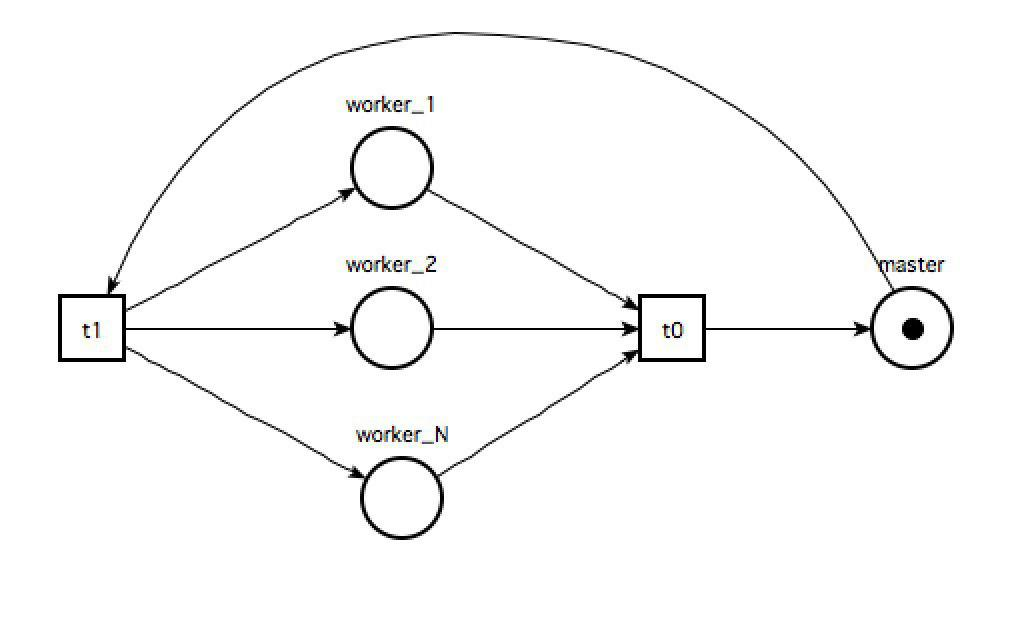
\includegraphics[width=10cm]{FIGURE/petrinet.jpg}\end{center}}
\caption{Petri Net con tre thread \label{petrinet}}
\end{figure}

Allo stato iniziale il master-thread possiede il controllo del flusso di esecuzione. Al termine della computazione ne notifica il successo ai worker-threads dando loro la possibilit� di procedere con il calcolo.\\
Successivamente, il sistema dovr� attendere il completamento dell'esecuzione degli N worker-threads per eseguire la transazione t0 e restituire la parola al master-thread. 